\documentclass[12pt,a4paper]{scrartcl}
\usepackage{ngerman}
\usepackage[utf8]{inputenc}
\usepackage[T1]{fontenc}
\usepackage{amsmath, amssymb}
\usepackage{graphicx}
\usepackage{color}
\definecolor{darkblue}{rgb}{0,0,.6}
\definecolor{darkred}{rgb}{.6,0,0}
\definecolor{darkgreen}{rgb}{0,.6,0}
\definecolor{lightblue}{rgb}{0.97,0.99,1}

\usepackage{listings}
\lstset{
  language=Python,
  basicstyle=\ttfamily,
  commentstyle=\color{darkgreen},
  keywordstyle=\bfseries\color{darkblue},
  stringstyle=\color{darkred},
  showspaces=false,
  showstringspaces=false,
  showtabs=false,
  columns=fixed,
  frame=single,
  numbers=left,
  numberstyle=\tiny,
  numbersep=5pt,
  breaklines=true,
  backgroundcolor=\color{lightblue},
  captionpos=b
}


\title{Dokumentation vom Teamprojekt}
\author{Alle}
\date{today}


\begin{document}
\maketitle
\tableofcontents

%\section{Einleitung}


%\section{Funktionsweise}


% Hier wird das Deployment beschrieben.
% --------------------------------------------------------------------

\chapter{Deployment}
\section{Frontend}
Folgende Pakete werden für die funktionsfähigkeit der Webseite benötigt:
  \begin{itemize}
	\item paramiko
	\item django 1.3
	\item django-registration
  \end{itemize}


Zuerst muss das Projekt geforkt werden. Dazu im gewünschten Ordner den Befehl '
git clone https://github.com/ctldev/ctlweb.git' ausführen. Im Ordner des
Projektes befindet sich im Subordner 'src/frontend' die manage.py von Django.
Hier sollte der Befehl 'python manage.py create\_impressum' ausgeführt werden,
um ein personalisiertes Impressum zu generieren. Alternativ muss ein eigenes 
in dem Ordner 'src/frontend/template' mit dem Namen
'personal\_impressum.html' generiert werden. Nun kann die Webseite gestartet
werden.
Auf der Webseite sollten nun in der Admin-Section die Cluster hinzugefügt werden,
auf denen sich die darzustellenden Komponenten befinden. Die Komponenten des
Clusters lassen sich über den Befehl 'python manage.py request\_modules'
abfragen. Regelmäßige Abfragen sind so auch zum Beispiel über einen Cron-Job
oder Ähnliches zu realisieren.
\section{Backend}
Folgendes Paket wird für die Funktionsfähigkeit des Programms benötigt:
\begin{itemize}
  \item requests (python3)
\end{itemize}

%
%diese datei fungiert jediglich als aufteilung der dokumentation
\section{Frontend}


\section{Backend}
Das Backend betreibt unabhängig vom Frontend eine eigene Datenbank und definiert
zusätzlich eigene Methoden, die die volle Kontrolle über diese DB bieten.
Weiterhin definiert das Backend einige Konsolen Befehle, welche die 
komfortable Nutzung sowie Administration von ctl-Systemen auf Clustern 
sowie von Nutzern ermöglicht.   
\subsection{Datenbankstruktur und ihre Zugriffsmethoden}
\begin{figure}[H]
  \begin{center}
	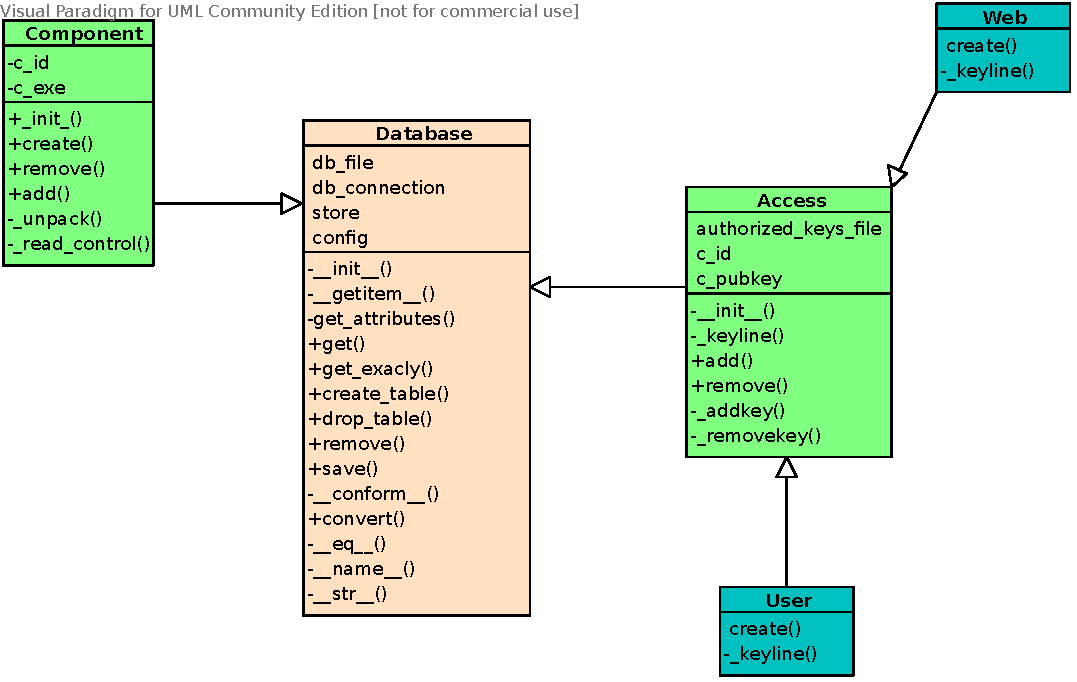
\includegraphics[width=\linewidth]{bilder/clsdiagrambackend.pdf}
	\caption{Klassen Diagramm der Datenbank}
	\label{g_bd_db}
  \end{center}
\end{figure}

Database ist die Vaterklasse. Sie besitzt alle wichtigen Methoden,
die nötig sind, um die Datenbank des Backends zu
betreiben(create(),save(),remove(),get()).

Component stellt die Tabelle \glqq Component\grqq\ in der DB dar und 
spezifiziert deren Attribute \glqq id\grqq\ und \grqq exe\grqq. Component 
erbt von Database, um ihre Tabelle zu modifizieren. Dazu kommen eigene 
Methoden, um Komponenten hochzuladen etc.

Access ist wichtig, um ssh Zugriffmodifikationen zu ermöglichen.
Alle Klassen, die dies möchten, werden von dieser Klasse abgeleitet.
Access erbt zudem von Database.

User und Web erben von Access und damit indirekt auch von Database.
Sie stellen die Tabelle User bzw. Web in der DB dar.

\subsection{Konsolen Befehle}
Folgende Konsolen Befehle existieren:
\begin{itemize}
  \item ctl-build
  \item ctl-genmanifest
  \item ctl-init
  \item ctl-register
  \item ctl-runcgi
  \item ctl-web
  \item ctl-webinteractive
\end{itemize}

\subsubsection{ctl-init}
ctl-init startet die gewünschte Komponente auf dem Cluster.

\subsubsection{ctl-genmanifest}
\begin{figure}[H]
  \begin{center}
	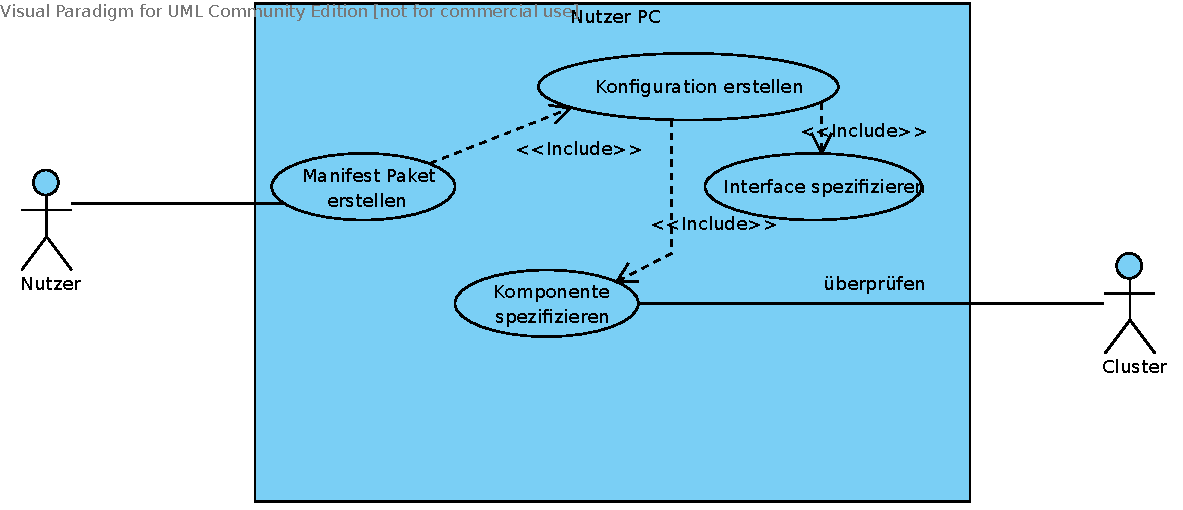
\includegraphics[scale=0.7]{bilder/ctl-genmanifest_usecase.pdf}
	\caption{Use-Case Diagramm von ctl-genmanifest}
	\label{g_ctl-genmanifest_uc}
  \end{center}
\end{figure}
Wie in Abb.\ \ref{g_ctl-genmanifest_uc} zu sehen, kann der Nutzer von seinem
Code ein Manifest Paket erstellen lassen, indem er die Komponente und dessen
Interface spezifiziert. Sobald der Cluster das o.k. gibt, wird das Manifest
Paket geschnürt.

\subsubsection{ctl-register / ctl-web}
\begin{figure}[H]
  \begin{center}
	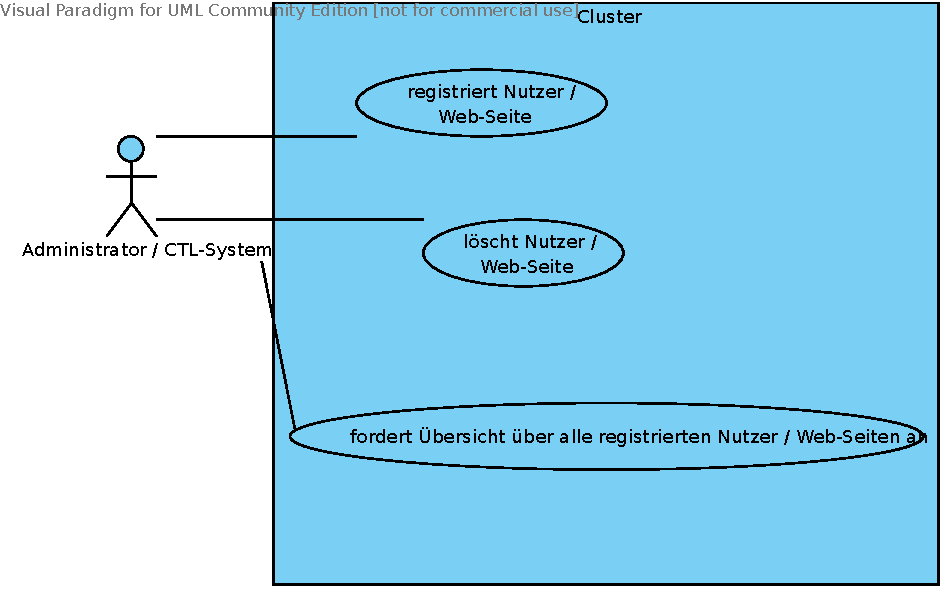
\includegraphics[scale=0.6]{bilder/ctl-register_usecase.pdf}
	\caption{Use-Case Diagramm von ctl-register / ctl-web}
	\label{g_ctl-register_uc}
  \end{center}
\end{figure}
In Abb.\ \ref{g_ctl-register_uc} ist ein Use Case dargestellt, welches
ctl-register und ctl-web in einem Diagramm zeigt, da beide Funktionen im Grunde  
die gleichen Dinge bewältigen.
Das ctl-System bzw. der Administrator kann Nutzer und/oder Web-Seiten
entweder registrieren oder löschen.
Eine Zusatzfunktion ist die Übersicht über alle registrierten Nutzer
und/oder Web-Seiten.

\subsubsection{ctl-webinteractive}
\begin{figure}[H]
  \begin{center}
	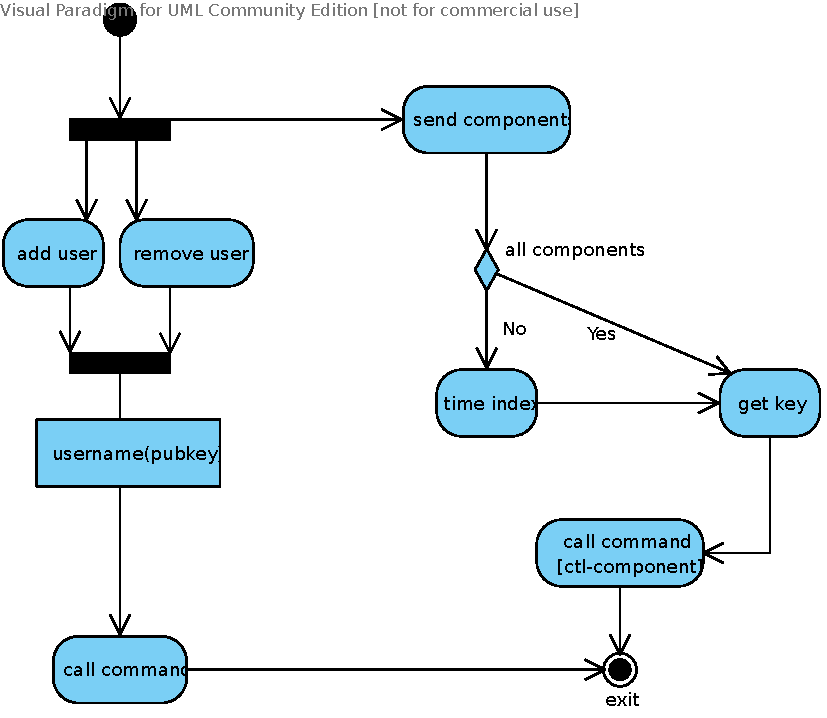
\includegraphics[scale=0.6]{bilder/activitydiagrambackend.pdf}
	\caption{Activity Diagramm von ctl-webinteractive}
	\label{g ctl-webinteractive}
  \end{center}
\end{figure}
ctl-webinteractive stellt einen besonderen Dienst zur Verfügung, und zwar
erlaubt es dem unerfahrenen Benutzer durch einen "`Wizard"' bestimmte Befehle
wie ctl-component, ctl-register sowie ctl-web ausführen. Der Nutzer wird dabei
durch jeden einzelnen Schritt geleitet, wie Namen, Key oder sonstiges eingeben.
Am Ende führt ctl-webinteractive dann den entsprechenden Befehl mit den
gegebenen Werten aus. Das Verhalten des ctl-webinteractive Befehls ist 
im Bild zu sehen \ref{g ctl-webinteractive}.


%\section{Schlusswort}
Hiermit endet die Dokumentation des ctl Systems.
Das Team hofft etwaige Fragen beantwortet zu haben und wünscht allen 
Nutzern sowie den Administratoren viel Spaß mit dem ctl System.
Bei Fragen steht ihnen unsere Team gerne zur Verfügung.



\end{document}

